\documentclass[a4paper,12pt,twoside]{report}

% Packages
\usepackage{graphicx} % -> Images, includegraphics command
\usepackage{amsmath} % -> Matrices, pmatrix command
\usepackage[cm]{fullpage}

% Other configuration
\graphicspath{ {./Resources/} }

\begin{document}

	\begin{abstract}
		Nowadays traffic in rush hours is crowded. The causes of this issue - besides the countless automobiles which is much more than the streets of cities were initially designed for - are inattention, hurrying and other distracting activities. This report purpose is to investigate the effect of autonomous drivers in the rush hour traffic with special attention to the red light situations.

		A literature review was accomplished to investigate the behavior of normal and autonomous drivers. Based on that it can be stated that traffic models can be divided into micro- and macroscopic models. Microscopic behaviors are more suitable to model red light situations, so the process was continued with these.

		The red light situations were simulated with a car following model. The algorithm used during the simulations was a combination of Intelligent Driver Model and the so called MOBIL model.

		Several simulations with various driver types (form the low reaction time old timer to the aggressive business man) were evaluated.

		The simulations showed that the effect of autonomous drivers is very positive in traffic. 
	\end{abstract}

	\tableofcontents

	\chapter{Introduction}
		Recently there is huge attention on self-driving cars. It seems that in a few years self-driving cars will hit the public roads. So it could be interesting that how much effect these cars will have on today's crowded streets. To find out a model should be developed to simulate real traffic situations without autonomous cars and then exchange real drivers one by one to `robots`. To develop a simulator that is capable of simulating real traffic behaviors It was a must to check out what has been already developed by the industry.

		There are several publications and even open source example implementations on this topic. Various traffic flow models have been developed like car following or hydrodynamic models. One of the main applications is that based on the traffic simulation results provided by these simulators, engineers can design better traffic systems. It can be also used to simulate stop and go traffic on the highways and suggest a speed limit based on that to avoid traffic jam. There are researches about improving traffic via network communications between cars and also with traffic lights. Theses researches also based on traffic simulators.
	\chapter{Traffic models}
		\section{Theory behind traffic simulators}
			One of the main branch of these algorithms are the so called macroscopic or hydrodynamic models. These deal with traffic as a fluid flow and they do not take individual driver actions into consideration. These are based on the vehicle density.

			The other type is the microscopic or car following models. These models do take individual driver behavior into consideration. So they are simulating each cars in a particular traffic situation. Some examples are the optimal velocity model, velocity difference model or the IDM. The task is to find a model that can accurately represent a human driven car. The model consists two parts, longitudinal and transversal movements. Although most of the simulations only care about the former one in this thesis both of them will be investigated.
		\section{Intelligent Driver Model description} \label{sec:IDM}
			One of the most widespread microscopic model is the Intelligent Driver Model. IDM is a time continuous car following model which belongs to the Optimal Velocity model family. IDM is designed to be accident-free. It can only represents longitudinal motions. The fundamental idea behind the model is that every car chooses its speed based on the car before and its individual parameters. In case when there is no car before then it can freely accelerate to its desired speed.

			IDM is defined by its acceleration function. The model is constructed by two parts. The first part represents the \textit{free acceleration} when there is no leading car or it is far away:
			\begin{equation}
				a_{free}=a_{max}\cdot \left [ 1 - \left ( \frac{v(t)}{v_d} \right )^\delta \right ]\,,
				\label{eq:afree}
			\end{equation}
			where
			\begin{itemize}
				\item $a_{\rm max}$ $\rm [m/s^2]$ is the maximum of the acceleration,
				\item $v(t)$ is the own velocity at $t$ in $\rm [m/s]$,
				\item $v_d$ is the desired velocity in $\rm [m/s]$,
				\item $\delta$ is the free acceleration exponent.
			\end{itemize}
			Equation \ref{eq:afree} produces zero when the current speed equals to the desired speed ($v(t)=v_d$) and it reaches its maximum value when the car is not moving ($v(t)=0$).
			The second part corresponds to the \textit{follower behavior} or \textit{breaking strategy} of the model:
			\begin{equation}
				a_{follower}=-a_{max}\cdot \left ( \frac{h_d(t)}{h(t)} \right )^2\,,
				\label{eq:afollower}
			\end{equation}
			where
			\begin{itemize}
				\item $h(t)$ is the gap at $t$ in $[m]$,
				\item $h_d(t)$ is the desired safe gap at $t$ in $[m]$.
			\end{itemize}
			The current gap at a given $t$ can be calculated from:
			\begin{equation}
				h(t)=x_l(t)-L_l - x(t)
			\end{equation}
			where $x_l(t)$ and $L_l$ is the position and length of the described car's leader car, $x(t)$ is the car's own position.
			The desired safe gap can be calculated from:
			\begin{equation}
				h_d(t)=h_0 + v(t)\cdot T + \frac{v(t)-v_l(t)}{2\cdot \sqrt{a_{max}\cdot b_{max}}}\,,
			\end{equation}
			where $h_0$ is the bumper to bumper gap or jam distance, $T$ is the desired safety time headway, $v_l(t)$ is the velocity of its leading car, $b_{max}$ is the maximum value of comfortable deceleration.
			Equation \ref{eq:afollower} will decreases with increasing own speed, increasing velocity difference and decreasing distance to the front car.
			\begin{figure}[ht]
				\centering
				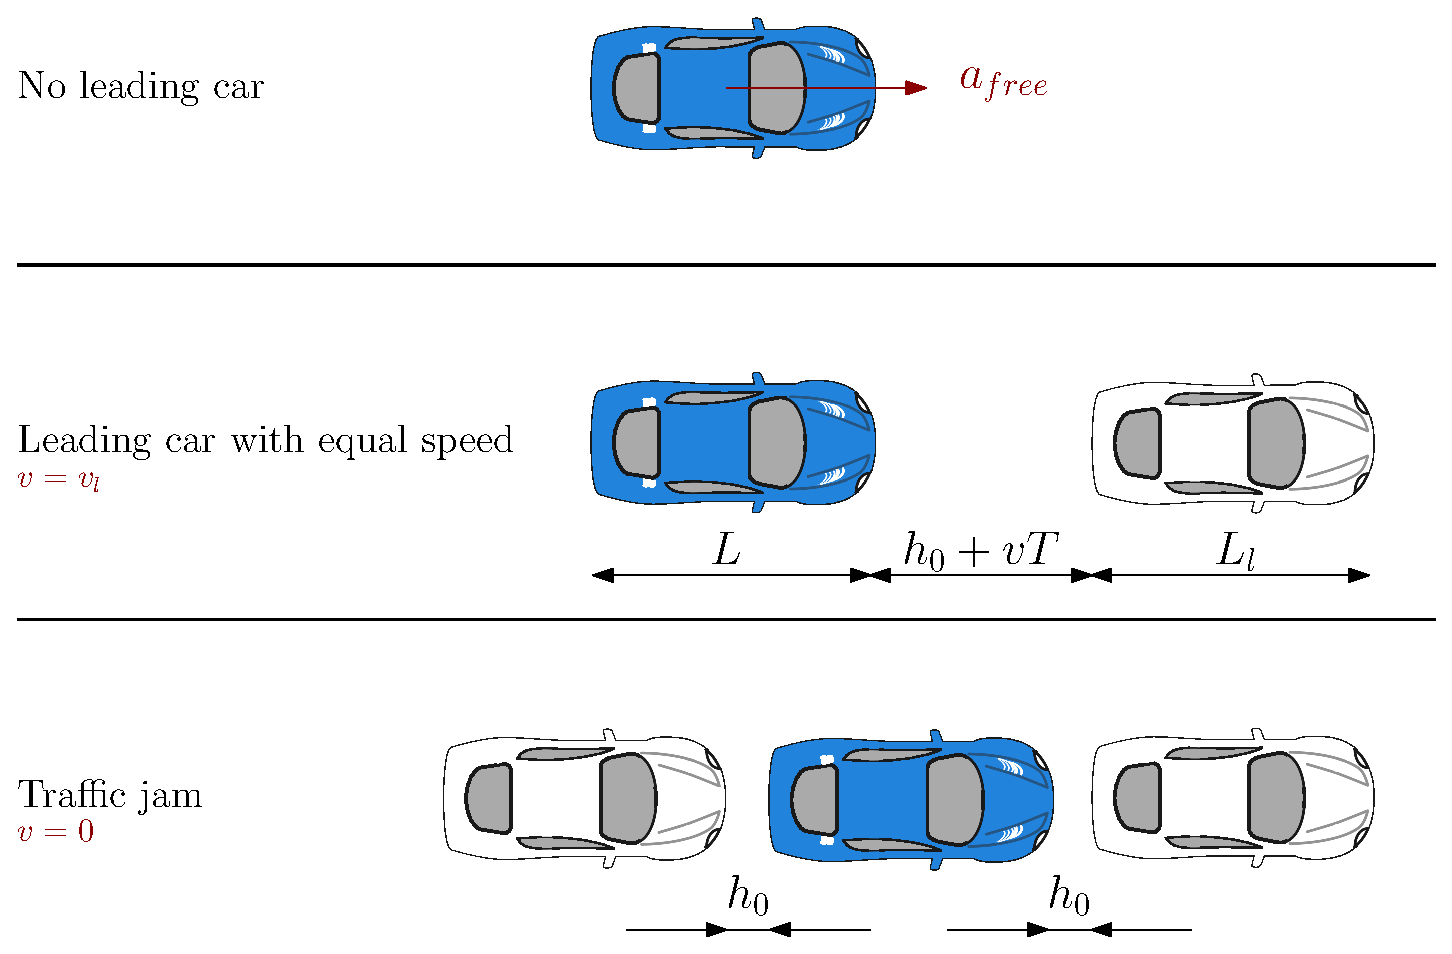
\includegraphics[width=.8\textwidth]{idm.eps}
				\caption{3 special case of IDM model}
				\label{fig:idm}
			\end{figure}
			The sum of equation \ref{eq:afree} and \ref{eq:afollower} is the IDM equation which reads as follows:
			\begin{equation}
				a(t)=a_{free}+a_{follower}=a_{max}\left [ 1 - \left ( \frac{v(t)}{v_d} \right )^\delta - \left ( \frac{h_d(t)}{h(t)} \right )^2 \right ]\,.
				\label{eq:aidm}
			\end{equation}
			Equation \ref{eq:aidm} represents the longitudinal behavior mechanism of a human driven car.
		\section{Mobil} \label{sec:MOBIL}
			Beside the IDM there is a need for transversal motion model of the cars, namely a lane changing model. It has not been studied nearly as exhaustive as longitudinal behaviors. However it can have great impact on the overall traffic flow so it is worth investigating. The model should be able to decide based on the local traffic conditions that changing lane is beneficial and safe to a specific driver or not. If both conditions met the model will start to change lanes.

			The first condition to satisfy is that lane changing should be safe. The model should check that how will a possible lane change effect the upstream vehicles in the target lane. Mobil states if the deceleration of the new follower car does not exceeds a given safe limit then it is safe. It can be expressed with an inequality as well:
			\begin{equation}
				\hat{a}_n\geq -b_{safe}\,,
			\end{equation}
			where $\hat{a}_n$ is the new follower car's acceleration if car $c$ changes lanes and $b_{safe}$ is a parameter of car $n$. This criterion ensures that the model remains accident free even for edge cases.
			\begin{figure}[ht]
				\centering
				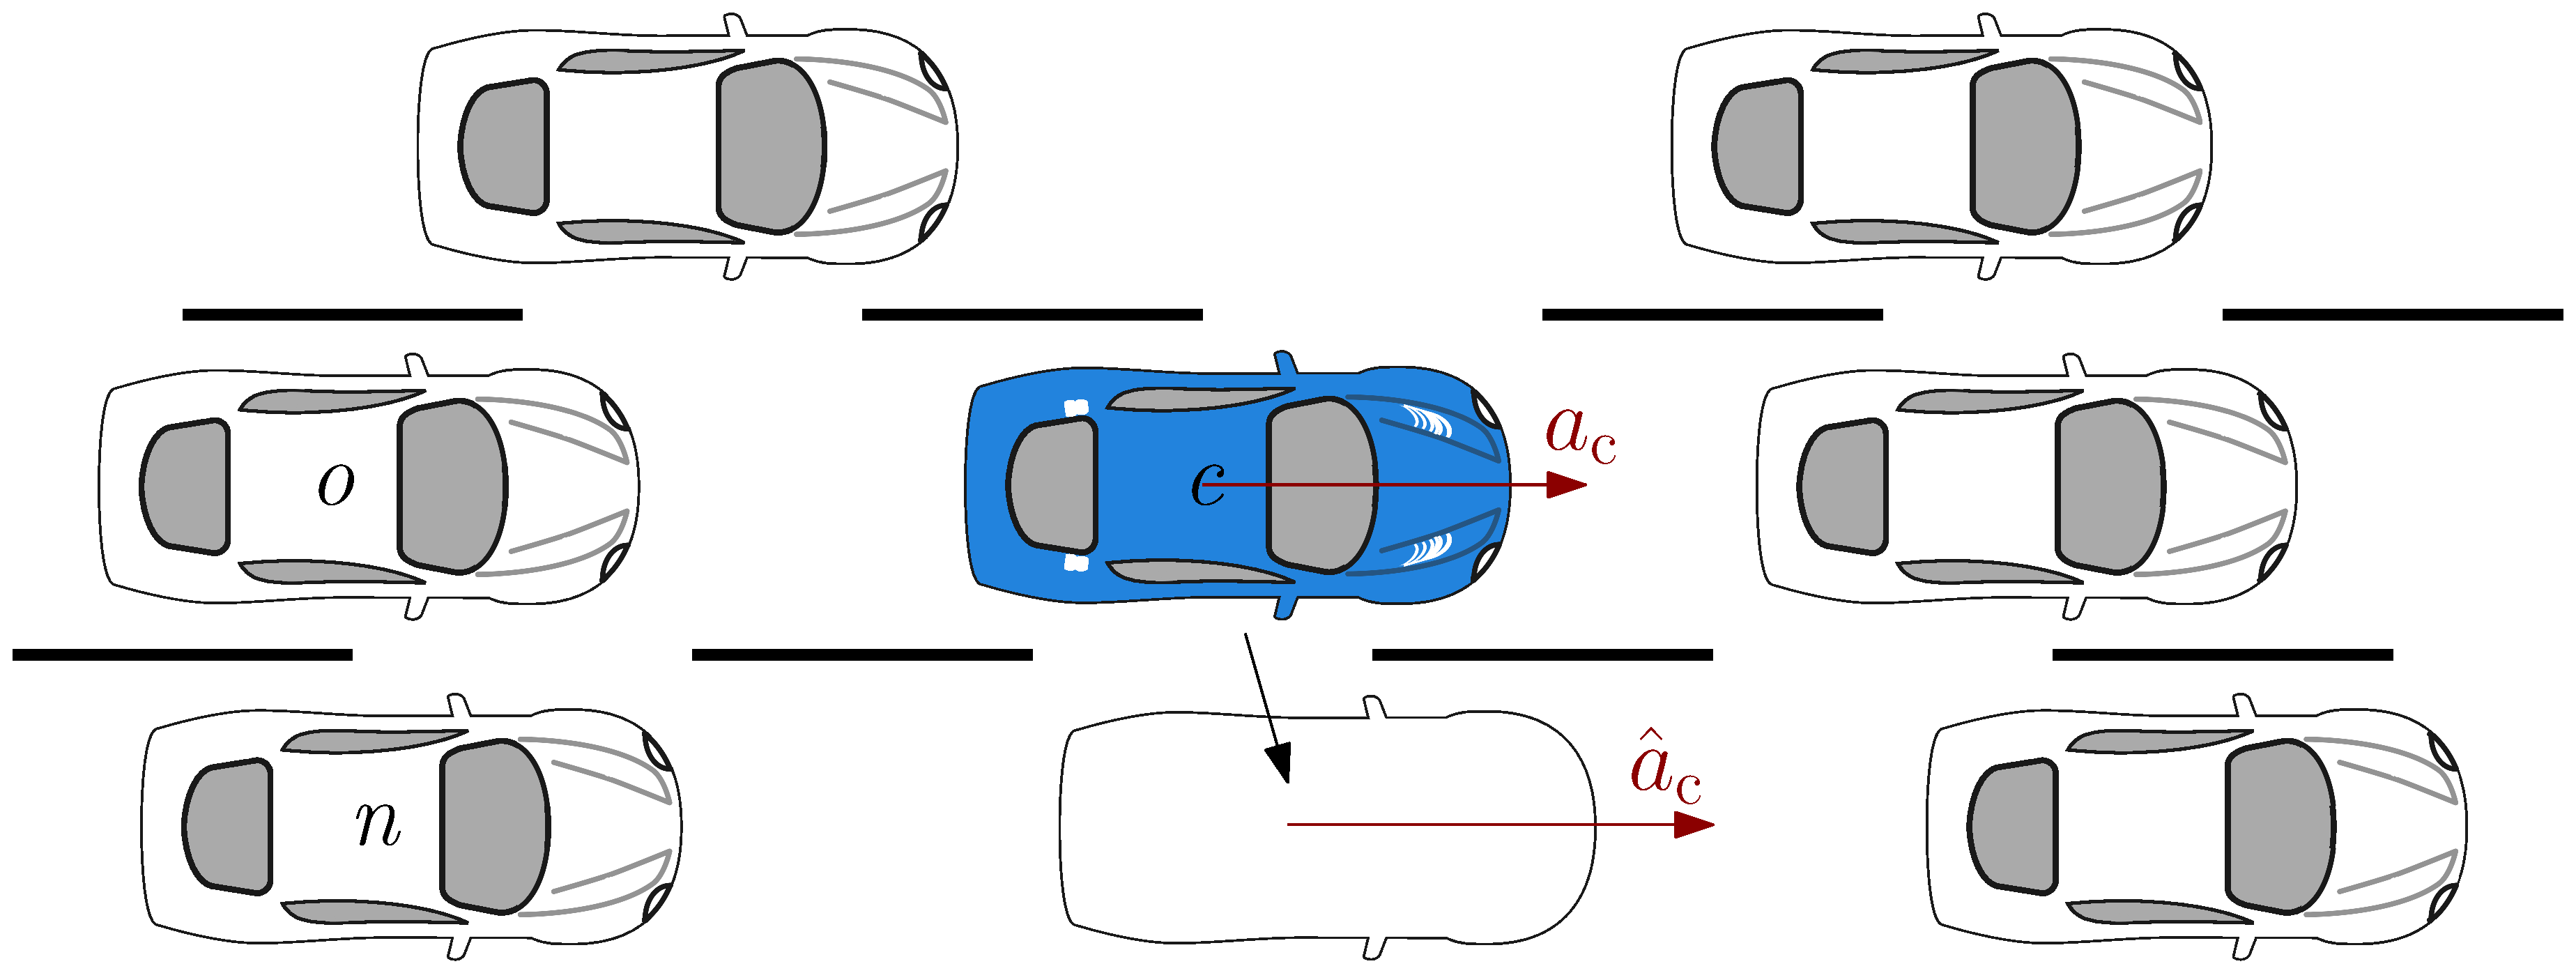
\includegraphics[width=\textwidth]{mobil.eps}
				\caption{Based on the local traffic conditions vehicle $c$ is considering changing lanes  to the right. Vehicle $n$ and $o$ will be the new and old followers of car $c$ respectively}
				\label{fig:mobil}
			\end{figure}
			The other condition is the incentive criterion which states that the lane change should improve the local traffic situation around the vehicle.  The base model is the following:
			\begin{equation}
				\hat{a}_c + \hat{a}_o + \hat{a}_n > a_c + a_o + a_n\,,
				\label{eq:mobil_first}
			\end{equation}
			where accelerations after a possible lane change are denoted with caps.
			Based on equation \ref{eq:mobil_first} a lane change should only occur if the sum of the accelerations after the lane change is greater than before. This inequality reflects the name of the model which is \textbf{m}inimizing \textbf{o}verall \textbf{b}raking \textbf{i}nduced by \textbf{l}ane change.

			However equation \ref{eq:mobil_first} is not as realistic as it should be. The first problem is that vehicles would change lanes  even for a negligible acceleration advantage which is not the case in a realistic traffic situation. This issue can be solved with a threshold value $\Delta  a_{th}$. After this modification equation \ref{eq:mobil_first} would look like below:
			\begin{equation}
				\hat{a}_c - a_c + \hat{a}_o - a_o + \hat{a}_n - a_n > \Delta  a_{th}\,,
				\label{eq:mobil_with_tr}
			\end{equation}
			It can be stated that with this modification individual drivers only change lanes if the acceleration sum is significantly greater than before the lane change. The other problem with the previously discussed models is that they can't distinguish between driving style. Driver styles can vary from complete selfish to the altruistic driver. Selfish drivers would only care about  their own acceleration ($\hat{a}_c - a_c > \Delta  a_{th}$) while altruistic ones would change lanes even if that would result in a disadvantageous position for them but with that change the local traffic situation is improved sufficiently ($\hat{a}_o - a_o + \hat{a}_n - a_n > \Delta  a_{th}$). A $p$ politeness factor should be introduced to fix that. Including $p$ in equation \ref{eq:mobil_with_tr} results in the final form of the model:
			\begin{equation}
				\hat{a}_c - a_c + p(\hat{a}_o - a_o + \hat{a}_n - a_n) > \Delta  a_{th}\,.
				\label{eq:mobil}
			\end{equation}
			A completely selfish driver would get $p=0$ factor, while an altruistic one $p>1$. In the special case where $p=1$ equation \ref{eq:mobil} simplifies back to equation \ref{eq:mobil_with_tr}, which means a lane change is performed only if the sum of all involved vehicles' acceleration will improved at least by the threshold value.
		\section{Numerical solver}
			In section \ref{sec:IDM} and \ref{sec:MOBIL} a vehicle behavior in traffic has been shown and modeled. The mathematical model of a driver is a second order differential equation. There is no analytical solution, so a numerical one should be carried out. To be able to use one of the common numerical solvers (like Explict Euler or 4th order Runge Kutta) the second order differential equation should be transformed into a first order differential equation system. So the second order differential equation is based on \ref{eq:aidm}:
			\begin{equation}
				\ddot{x}=a_{max}\left [ 1 - \left ( \frac{\dot{x}}{v_d} \right )^\delta - \left ( \frac{h_0 + \dot{x}\cdot T + \frac{\dot{x}-v_l}{c}}{x_l-L_l - x} \right )^2 \right ]\,.
				\label{eq:idm_num1}
			\end{equation}
			Let's say
			\begin{equation}
				y=
				\begin{pmatrix}
					y_1\\
					y_2
				\end{pmatrix}
				=
				\begin{pmatrix}
					x\\
					\dot{x}
				\end{pmatrix}\,,
				\label{eq:idm_num2}
			\end{equation}
			then the derivative of $y$ would be
			\begin{equation}
				\dot{y}=
				\begin{pmatrix}
					\dot{y_1}\\
					\dot{y_2}
				\end{pmatrix}
				=
				\begin{pmatrix}
					\dot{x}\\
					\ddot{x}
				\end{pmatrix}\,,
				\label{eq:idm_num3}
			\end{equation}
			From equations \ref{eq:idm_num1}, \ref{eq:idm_num2} and \ref{eq:idm_num3} it can be concluded that the differential equation system will be the following:
			\begin{equation}
				\dot{y}=
				\begin{pmatrix}
					y_2\\
					a_{max}\left [ 1 - \left ( \frac{y_2}{v_d} \right )^\delta - \left ( \frac{h_0 + y_2\cdot T + \frac{y_2-v_l}{c}}{x_l-L_l - y_1} \right )^2 \right ]
				\end{pmatrix}
				\label{eq:numerical_idm}
			\end{equation}
	\chapter{Evolution of the simulator}
			Equation \ref{eq:numerical_idm} can be solved with an Explicit Euler. To test the model a basic setup was implemented in MATLAB. The visual representation of the setup can be seen on figure \ref{fig:basic2car}.
			\begin{figure}[ht]
				\centering
				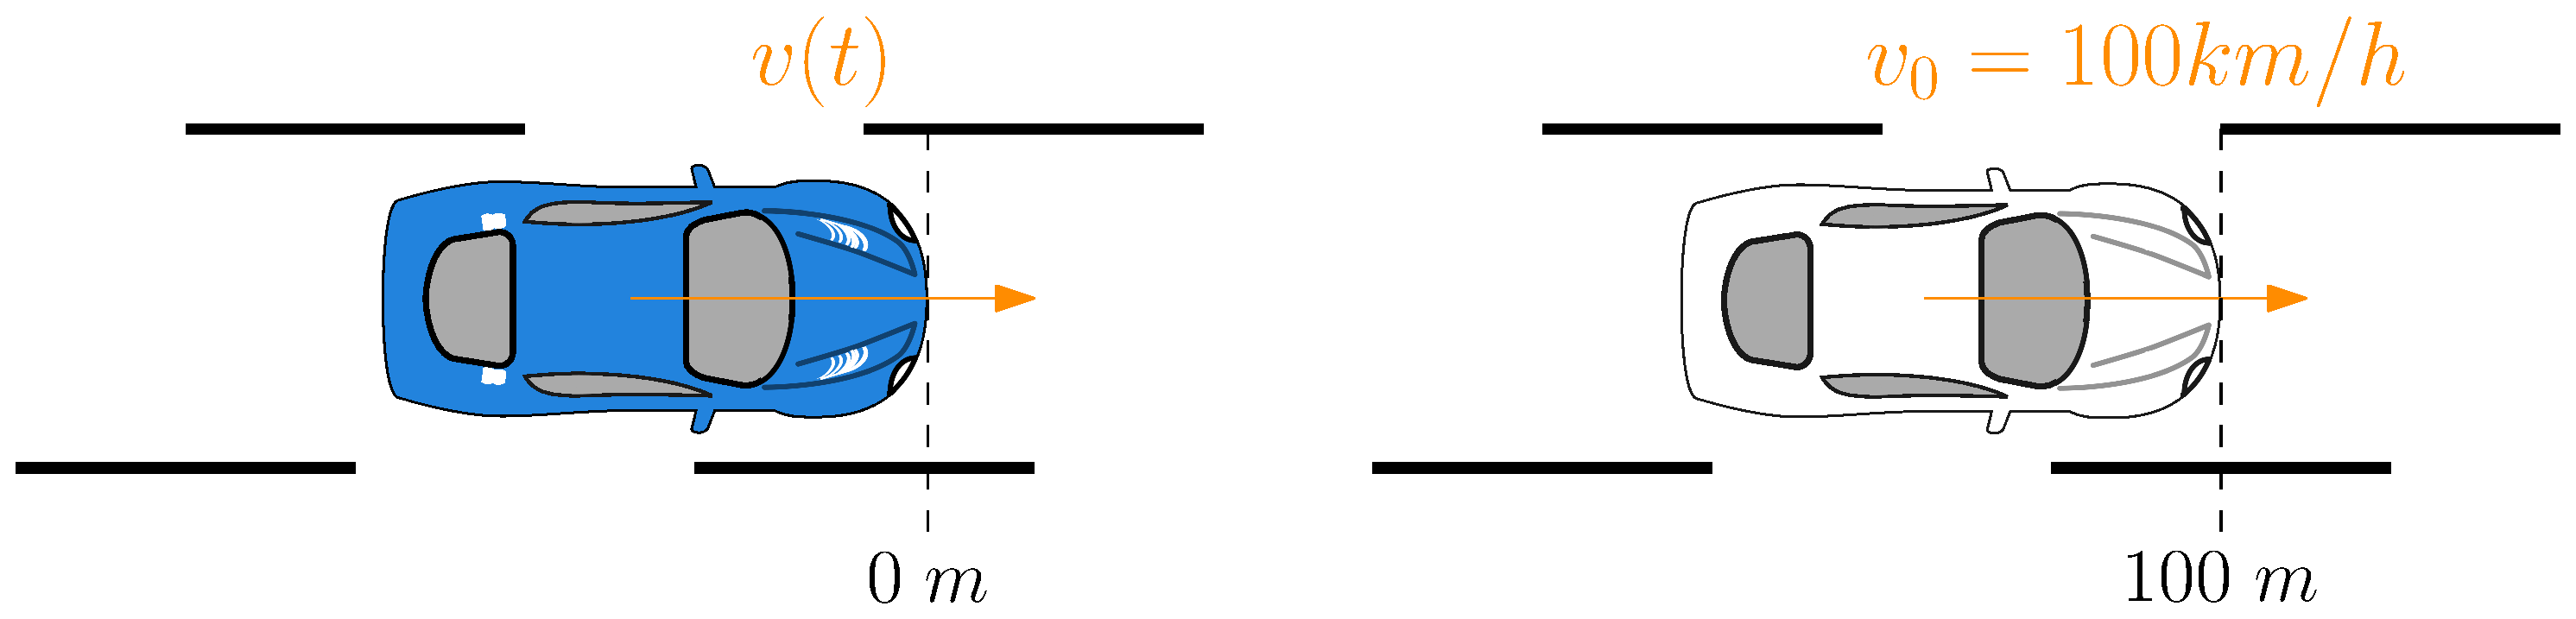
\includegraphics[width=\textwidth]{basic_2_car.eps}
				\caption{Basic setup with 2 cars}
				\label{fig:basic2car}
			\end{figure}
			The leading car has a constant $100\;km/h$ velocity. The following car which is modeled with IDM has an initial velocity of $100\;km/h$ as well. The parameters of following car can be seen in Table \ref{table:idm_params}
			\begin{figure}[ht]
				\begin{center}
					\begin{tabular}{ |c|c|c| } 
						\hline
						$a_{max}$ & $1.5$ & $m/s^2$ \\
						$b_{max}$ & $1.67$ & $m/s^2$ \\
						$v_d$ & $130$ & $km/h$ \\
						$T$ & $1.8$ & $s$ \\
						$h_0$ & $2$ & $m$ \\
						$\delta$ & $4$ & $-$ \\
						$L$ & $4.5$ & $m$ \\
						\hline
					\end{tabular}
				\end{center}
				\caption{Intelligent Driver Model parameters}
				\label{table:idm_params}
			\end{figure}
	\chapter{Final model}
		\section{Time step independence}
\end{document}
